% Options for packages loaded elsewhere
\PassOptionsToPackage{unicode}{hyperref}
\PassOptionsToPackage{hyphens}{url}
%
\documentclass[
]{article}
\usepackage{amsmath,amssymb}
\usepackage{iftex}
\ifPDFTeX
  \usepackage[T1]{fontenc}
  \usepackage[utf8]{inputenc}
  \usepackage{textcomp} % provide euro and other symbols
\else % if luatex or xetex
  \usepackage{unicode-math} % this also loads fontspec
  \defaultfontfeatures{Scale=MatchLowercase}
  \defaultfontfeatures[\rmfamily]{Ligatures=TeX,Scale=1}
\fi
\usepackage{lmodern}
\ifPDFTeX\else
  % xetex/luatex font selection
\fi
% Use upquote if available, for straight quotes in verbatim environments
\IfFileExists{upquote.sty}{\usepackage{upquote}}{}
\IfFileExists{microtype.sty}{% use microtype if available
  \usepackage[]{microtype}
  \UseMicrotypeSet[protrusion]{basicmath} % disable protrusion for tt fonts
}{}
\makeatletter
\@ifundefined{KOMAClassName}{% if non-KOMA class
  \IfFileExists{parskip.sty}{%
    \usepackage{parskip}
  }{% else
    \setlength{\parindent}{0pt}
    \setlength{\parskip}{6pt plus 2pt minus 1pt}}
}{% if KOMA class
  \KOMAoptions{parskip=half}}
\makeatother
\usepackage{xcolor}
\usepackage[margin=1in]{geometry}
\usepackage{color}
\usepackage{fancyvrb}
\newcommand{\VerbBar}{|}
\newcommand{\VERB}{\Verb[commandchars=\\\{\}]}
\DefineVerbatimEnvironment{Highlighting}{Verbatim}{commandchars=\\\{\}}
% Add ',fontsize=\small' for more characters per line
\usepackage{framed}
\definecolor{shadecolor}{RGB}{248,248,248}
\newenvironment{Shaded}{\begin{snugshade}}{\end{snugshade}}
\newcommand{\AlertTok}[1]{\textcolor[rgb]{0.94,0.16,0.16}{#1}}
\newcommand{\AnnotationTok}[1]{\textcolor[rgb]{0.56,0.35,0.01}{\textbf{\textit{#1}}}}
\newcommand{\AttributeTok}[1]{\textcolor[rgb]{0.13,0.29,0.53}{#1}}
\newcommand{\BaseNTok}[1]{\textcolor[rgb]{0.00,0.00,0.81}{#1}}
\newcommand{\BuiltInTok}[1]{#1}
\newcommand{\CharTok}[1]{\textcolor[rgb]{0.31,0.60,0.02}{#1}}
\newcommand{\CommentTok}[1]{\textcolor[rgb]{0.56,0.35,0.01}{\textit{#1}}}
\newcommand{\CommentVarTok}[1]{\textcolor[rgb]{0.56,0.35,0.01}{\textbf{\textit{#1}}}}
\newcommand{\ConstantTok}[1]{\textcolor[rgb]{0.56,0.35,0.01}{#1}}
\newcommand{\ControlFlowTok}[1]{\textcolor[rgb]{0.13,0.29,0.53}{\textbf{#1}}}
\newcommand{\DataTypeTok}[1]{\textcolor[rgb]{0.13,0.29,0.53}{#1}}
\newcommand{\DecValTok}[1]{\textcolor[rgb]{0.00,0.00,0.81}{#1}}
\newcommand{\DocumentationTok}[1]{\textcolor[rgb]{0.56,0.35,0.01}{\textbf{\textit{#1}}}}
\newcommand{\ErrorTok}[1]{\textcolor[rgb]{0.64,0.00,0.00}{\textbf{#1}}}
\newcommand{\ExtensionTok}[1]{#1}
\newcommand{\FloatTok}[1]{\textcolor[rgb]{0.00,0.00,0.81}{#1}}
\newcommand{\FunctionTok}[1]{\textcolor[rgb]{0.13,0.29,0.53}{\textbf{#1}}}
\newcommand{\ImportTok}[1]{#1}
\newcommand{\InformationTok}[1]{\textcolor[rgb]{0.56,0.35,0.01}{\textbf{\textit{#1}}}}
\newcommand{\KeywordTok}[1]{\textcolor[rgb]{0.13,0.29,0.53}{\textbf{#1}}}
\newcommand{\NormalTok}[1]{#1}
\newcommand{\OperatorTok}[1]{\textcolor[rgb]{0.81,0.36,0.00}{\textbf{#1}}}
\newcommand{\OtherTok}[1]{\textcolor[rgb]{0.56,0.35,0.01}{#1}}
\newcommand{\PreprocessorTok}[1]{\textcolor[rgb]{0.56,0.35,0.01}{\textit{#1}}}
\newcommand{\RegionMarkerTok}[1]{#1}
\newcommand{\SpecialCharTok}[1]{\textcolor[rgb]{0.81,0.36,0.00}{\textbf{#1}}}
\newcommand{\SpecialStringTok}[1]{\textcolor[rgb]{0.31,0.60,0.02}{#1}}
\newcommand{\StringTok}[1]{\textcolor[rgb]{0.31,0.60,0.02}{#1}}
\newcommand{\VariableTok}[1]{\textcolor[rgb]{0.00,0.00,0.00}{#1}}
\newcommand{\VerbatimStringTok}[1]{\textcolor[rgb]{0.31,0.60,0.02}{#1}}
\newcommand{\WarningTok}[1]{\textcolor[rgb]{0.56,0.35,0.01}{\textbf{\textit{#1}}}}
\usepackage{longtable,booktabs,array}
\usepackage{calc} % for calculating minipage widths
% Correct order of tables after \paragraph or \subparagraph
\usepackage{etoolbox}
\makeatletter
\patchcmd\longtable{\par}{\if@noskipsec\mbox{}\fi\par}{}{}
\makeatother
% Allow footnotes in longtable head/foot
\IfFileExists{footnotehyper.sty}{\usepackage{footnotehyper}}{\usepackage{footnote}}
\makesavenoteenv{longtable}
\usepackage{graphicx}
\makeatletter
\def\maxwidth{\ifdim\Gin@nat@width>\linewidth\linewidth\else\Gin@nat@width\fi}
\def\maxheight{\ifdim\Gin@nat@height>\textheight\textheight\else\Gin@nat@height\fi}
\makeatother
% Scale images if necessary, so that they will not overflow the page
% margins by default, and it is still possible to overwrite the defaults
% using explicit options in \includegraphics[width, height, ...]{}
\setkeys{Gin}{width=\maxwidth,height=\maxheight,keepaspectratio}
% Set default figure placement to htbp
\makeatletter
\def\fps@figure{htbp}
\makeatother
\setlength{\emergencystretch}{3em} % prevent overfull lines
\providecommand{\tightlist}{%
  \setlength{\itemsep}{0pt}\setlength{\parskip}{0pt}}
\setcounter{secnumdepth}{-\maxdimen} % remove section numbering
% definitions for citeproc citations
\NewDocumentCommand\citeproctext{}{}
\NewDocumentCommand\citeproc{mm}{%
  \begingroup\def\citeproctext{#2}\cite{#1}\endgroup}
\makeatletter
 % allow citations to break across lines
 \let\@cite@ofmt\@firstofone
 % avoid brackets around text for \cite:
 \def\@biblabel#1{}
 \def\@cite#1#2{{#1\if@tempswa , #2\fi}}
\makeatother
\newlength{\cslhangindent}
\setlength{\cslhangindent}{1.5em}
\newlength{\csllabelwidth}
\setlength{\csllabelwidth}{3em}
\newenvironment{CSLReferences}[2] % #1 hanging-indent, #2 entry-spacing
 {\begin{list}{}{%
  \setlength{\itemindent}{0pt}
  \setlength{\leftmargin}{0pt}
  \setlength{\parsep}{0pt}
  % turn on hanging indent if param 1 is 1
  \ifodd #1
   \setlength{\leftmargin}{\cslhangindent}
   \setlength{\itemindent}{-1\cslhangindent}
  \fi
  % set entry spacing
  \setlength{\itemsep}{#2\baselineskip}}}
 {\end{list}}
\usepackage{calc}
\newcommand{\CSLBlock}[1]{\hfill\break\parbox[t]{\linewidth}{\strut\ignorespaces#1\strut}}
\newcommand{\CSLLeftMargin}[1]{\parbox[t]{\csllabelwidth}{\strut#1\strut}}
\newcommand{\CSLRightInline}[1]{\parbox[t]{\linewidth - \csllabelwidth}{\strut#1\strut}}
\newcommand{\CSLIndent}[1]{\hspace{\cslhangindent}#1}
\ifLuaTeX
  \usepackage{selnolig}  % disable illegal ligatures
\fi
\usepackage{bookmark}
\IfFileExists{xurl.sty}{\usepackage{xurl}}{} % add URL line breaks if available
\urlstyle{same}
\hypersetup{
  pdftitle={Mendelian Randomization},
  hidelinks,
  pdfcreator={LaTeX via pandoc}}

\title{Mendelian Randomization}
\author{}
\date{\vspace{-2.5em}2025-01-08}

\begin{document}
\maketitle

\subsection{Background}\label{background}

Mendelian randomization (MR) is used when it is either not possible or
unethical to conduct randomized controlled trials. In essence MR uses
genetic variants, such as single-nucleotide polymorphisms (SNPs), to
estimate the causal effect on an outcome. The genetic variants are used
since they are randomly allocated to individuals before any exposure or
outcome, which eliminates many confounding factors. In the setting of MR
genetic variants are also called instruments/instrumental variables. In
this document they are called genetic instrument.

There are three core assumptions for the genetic instruments
(\citeproc{ref-bowden2015}{Bowden, Smith, and Burgess 2015};
\citeproc{ref-sekula2016}{Sekula et al. 2016}). These are:

\begin{enumerate}
\def\labelenumi{\arabic{enumi}.}
\tightlist
\item
  It must be reproducibly and strongly associated with the exposure
\item
  It must not be associated with any known confounding factors
\item
  It must not be associated with the outcome except through the exposure
  (\citeproc{ref-bowden2015}{Bowden, Smith, and Burgess 2015};
  \citeproc{ref-sekula2016}{Sekula et al. 2016}).
\end{enumerate}

\begin{figure}
\centering
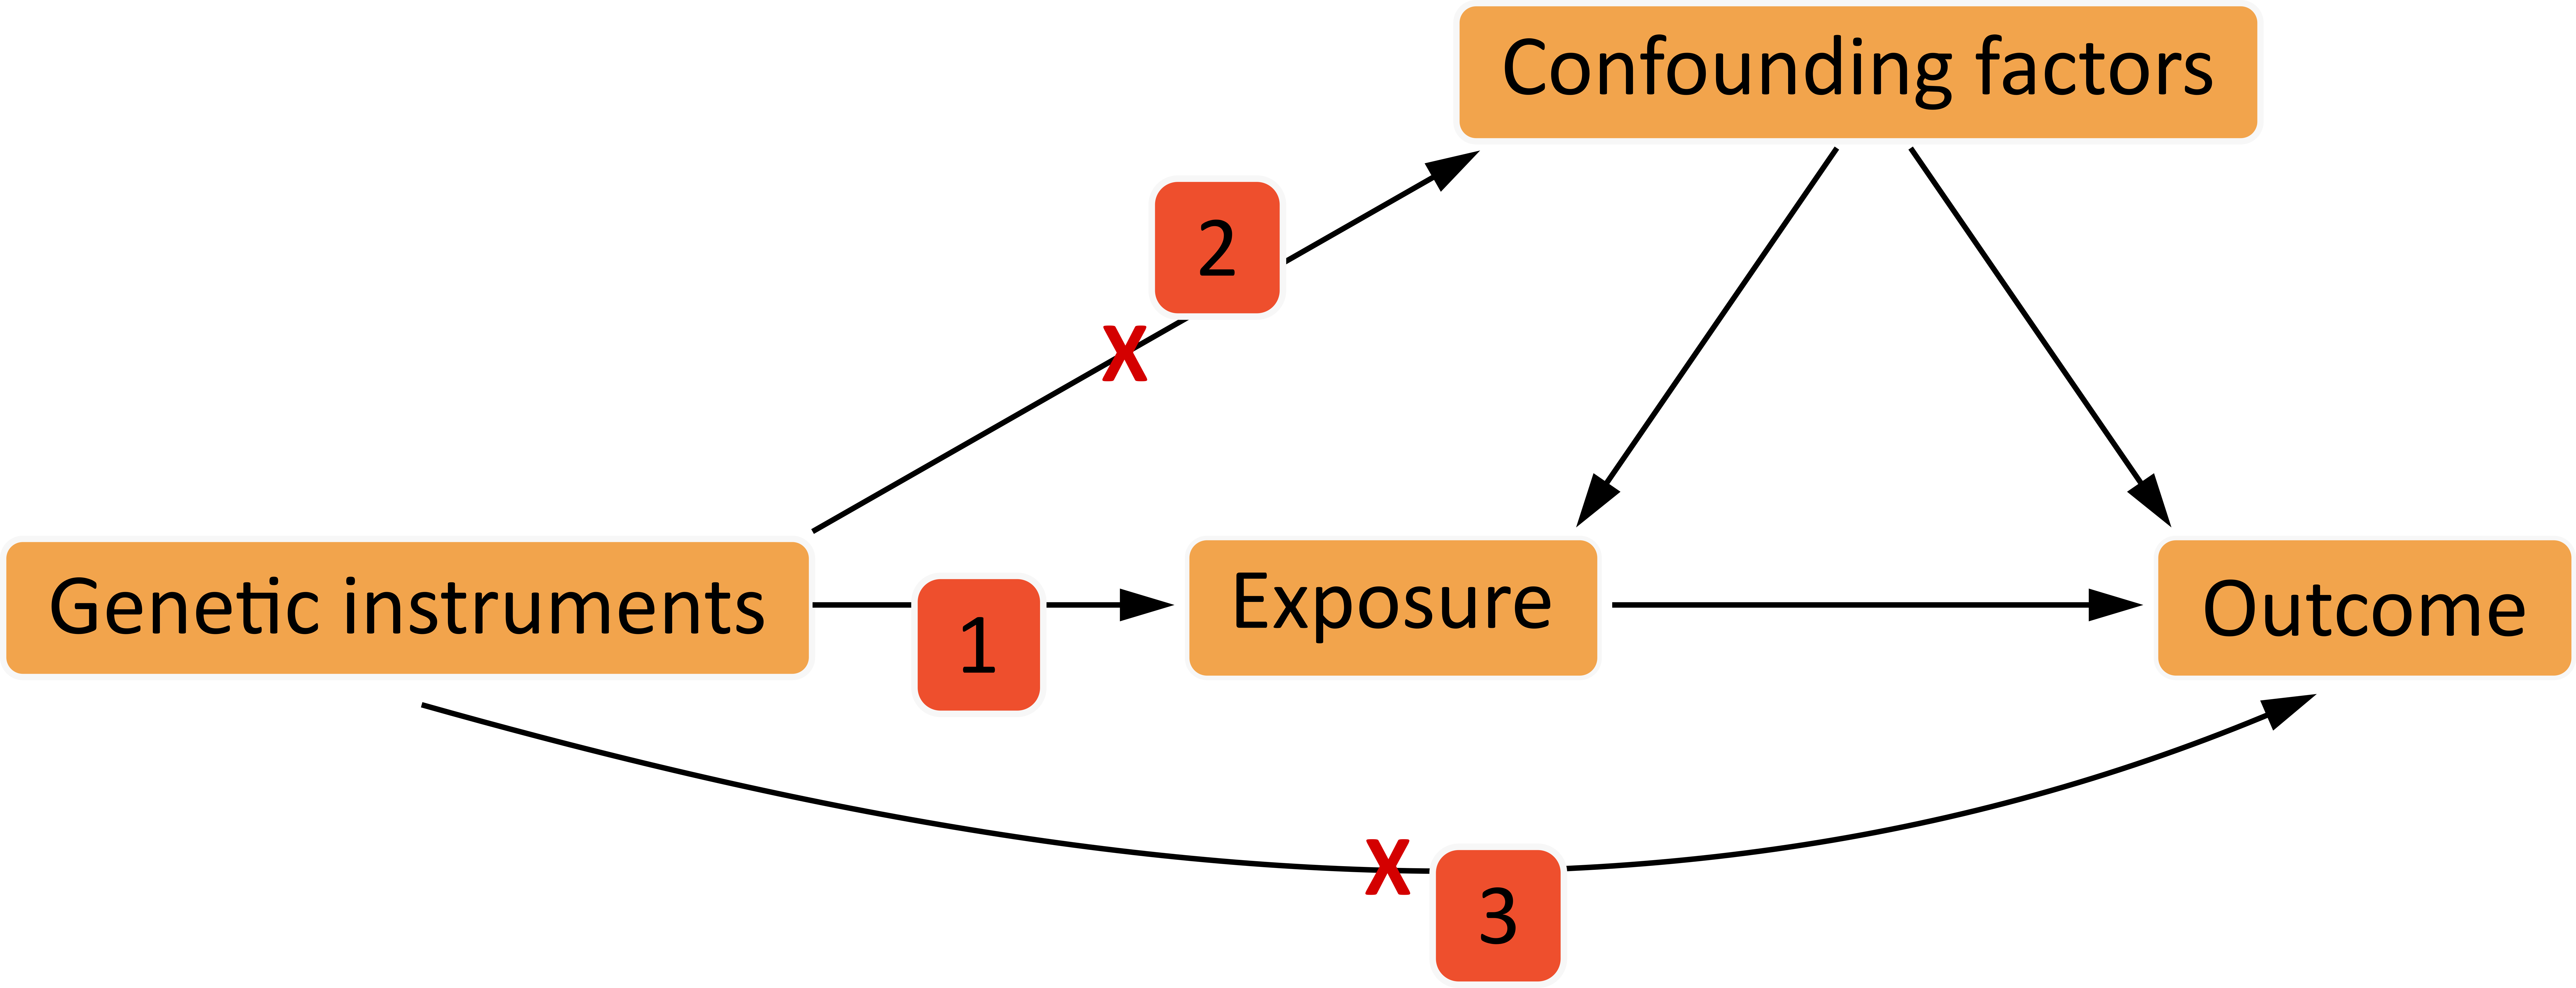
\includegraphics[width=0.5\textwidth,height=\textheight]{C:/Users/sarar/OneDrive/Skrivebord/Virksomhedspraktik/Mendelian-randomization2_figures/MR_analysis_assumptions.png}
\caption{A schematic overview of MR analysis and its assumptions:
\textbf{Assumption 1:} The instrument is reproducibly and strongly
associated with the exposure. \textbf{Assumption 2:} The instrument is
not associated with any known confounding factors. \textbf{Assumption
3:} The instrument is not associated with the outcome except through the
exposure (\citeproc{ref-bowden2015}{Bowden, Smith, and Burgess 2015};
\citeproc{ref-sekula2016}{Sekula et al. 2016}). \label{assumptions}}
\end{figure}

The first assumption can be investigated and proven either right or
wrong, but the second and third assumption cannot. Therefore some
statistical methods for MR have taken this into consideration, but they
have other assumptions:

\begin{enumerate}
\def\labelenumi{\arabic{enumi}.}
\setcounter{enumi}{3}
\tightlist
\item
  \textbf{InSIDE assumption:} Instrument Strength Independent of Direct
  Effects: The pleiotropic effects must be distributed independently of
  the instrument strength (\citeproc{ref-bowden2015}{Bowden, Smith, and
  Burgess 2015}; \citeproc{ref-bowden2016}{Bowden et al. 2016};
  \citeproc{ref-hartwig2017}{Hartwig, Smith, and Bowden 2017}).
\item
  \textbf{ZEMPA assumption:} ZEro Modal Pleiotropy Assumption: Across
  all instruments the most frequent value of the bias term is 0 \(\to\)
  the most common causal effect estimate is a consistent estimate of the
  true causal effect, even if the majority of instrumetns are invalid
  (\citeproc{ref-hartwig2017}{Hartwig, Smith, and Bowden 2017}).
\end{enumerate}

There are several steps of an MR analysis:

\begin{enumerate}
\def\labelenumi{\arabic{enumi}.}
\tightlist
\item
  Define the presumed causal association of interest
\item
  Choose at least one genetic variant to use as the genetic instrument

  \begin{itemize}
  \tightlist
  \item
    The stronger the genetic instrument is associated with the exposure,
    the stronger the power is. If the association is not strong enough
    to reach the required power, more can be used, but this increases
    the risk of bias, since it increases the risk of including invalid
    instruments.
  \end{itemize}
\item
  Evaluate core assumptions and discuss their applicability
\item
  Carry out the statistical MR analysis

  \begin{itemize}
  \tightlist
  \item
    The statistical MR analysis depends on the available data \(\to\) is
    the data individual level or summary? Is it a one sample or two
    sample MR analysis? Are there one or more genetic instruments?
  \end{itemize}
\item
  Interpret and discuss results (\citeproc{ref-sekula2016}{Sekula et al.
  2016}).
\end{enumerate}

As mentioned above some of the confounding factors of randomized
controlled studies are avoided in MR analysis, but MR still has some
limitations and possible confounding factors, these are:

\begin{itemize}
\tightlist
\item
  \textbf{Low statistical power:} MR studies can have low power if the
  sample size is too small or the genetic instrument does not account
  for enough of the investigated association
  (\citeproc{ref-smith2014}{Smith and Hemani 2014}).
\item
  \textbf{Reverse causation} the genetic instrument may cause the
  disease outcome, which causes the biomarker or the causal direction
  may be in the opposite direcetion (\citeproc{ref-smith2014}{Smith and
  Hemani 2014}).
\item
  \textbf{Population stratification:} The allele frequencies and disease
  exposure rates may vary between different subgroups of the population,
  which may lead to confounding (\citeproc{ref-sekula2016}{Sekula et al.
  2016}).
\item
  \textbf{Reintroduced confounding through pleiotropy:} The gentic
  instrument is associated with more than one apparently unrelated trait
  or disease - it influences more than one post-transcriptional process,
  which leads to confounding (\citeproc{ref-sekula2016}{Sekula et al.
  2016}; \citeproc{ref-smith2014}{Smith and Hemani 2014}).
\item
  \textbf{Linkage disequilibrium (LD) induced confounding:} The
  non-random association between different genetic variants on the same
  chromosomes, which leads to confounding if LD leads to the association
  of genetic instruments related to more than one post-transcriptional
  process (\citeproc{ref-sekula2016}{Sekula et al. 2016};
  \citeproc{ref-smith2014}{Smith and Hemani 2014}).
\item
  \textbf{Canalization/developmental compensation:} Compensatory
  developmental processes buffers the effect of genetic instruments that
  leads to potentially disruptive influences
  (\citeproc{ref-sekula2016}{Sekula et al. 2016}).
\item
  \textbf{Lack of genetic instruments to proxy for modifiable exposure
  interest:} If there is no reliable genetic instrument associated with
  the exposure, the MR cannot be performed
  (\citeproc{ref-smith2014}{Smith and Hemani 2014}).
\item
  \textbf{Complexity of associations:} If there is not enough biological
  knowledge regarding the genetic instrument, the exposure, the outcome
  and the associations of these, wrong conclusions may be drawn from the
  analysis (\citeproc{ref-smith2014}{Smith and Hemani 2014}).
\item
  \textbf{Weak instruments:} If the association between the genetic
  instrument and the exposure is weak, the exposure-outcome association
  may be biased and therefore the genetic instrument may give misleading
  results (\citeproc{ref-sekula2016}{Sekula et al. 2016}).
\end{itemize}

Therefore it is best to use a genetic instrument with a functional
association to the exposure/a genetic instrument that is located in
genes with biologic functions that are well known so it is more simple
to assess whether or not the assumptions are met
(\citeproc{ref-sekula2016}{Sekula et al. 2016}).

There are several types of MR studies/analyses some of these are
one-sample MR, two-sample MR, network MR and bidirectional MR. This
document will focus on the two-sample MR analysis using summary data.
Here two individual samples are used where one has the measurements for
the exposure, and the other has the measurements for the outcome. Both
samples have the same genetic instruments
(\citeproc{ref-boehm2022}{Boehm and Zhou 2022}). When performing a
two-sample MR study one has to consider two additional assumptions:

\begin{itemize}
\tightlist
\item
  The two samples must represent the same underlying population.
\item
  There is no overlap in participants between the two samples
  (\citeproc{ref-davies2018}{Davies, Holmes, and Smith 2018}).
\end{itemize}

When a presumed causal association of interest has been chosen the rest
of the MR analysis can be performed in R using the Two Sample MR
analysis package (\citeproc{ref-twosamplemr}{Hemani et al. 2018};
\citeproc{ref-mrsteiger}{Hemani, Tilling, and Davey Smith 2017}). The
Two Sample MR analysis package uses the following statistical methods:

\begin{itemize}
\tightlist
\item
  Wald Method
\item
  Inverse Variance Weighting (IVW)
\item
  Weighted Median Estimator
\item
  MR-Egger
\item
  Simple mode
\item
  Weighted mode (\citeproc{ref-twosamplemr}{Hemani et al. 2018};
  \citeproc{ref-mrsteiger}{Hemani, Tilling, and Davey Smith 2017}).
\end{itemize}

Each method has its own weaknesses and strengths. (They may be performed
all at once to see if they `agree' but one should be aware if the
assumptions for the specific method is met.) An overview of some of the
limitations of these methods can be seen in the figure below.

\begin{figure}
\centering
\includegraphics[width=0.75\textwidth,height=\textheight]{C:/Users/sarar/OneDrive/Skrivebord/Virksomhedspraktik/Mendelian-randomization2_figures/MR_analysis_flow2.png}
\caption{An overview of some of the statistical methods for two-sample
MR analysis: \textbf{Breakdown level:} The percent of variants that can
be invalid, while still providing a consistent estimate
(\citeproc{ref-boehm2022}{Boehm and Zhou 2022};
\citeproc{ref-hartwig2017}{Hartwig, Smith, and Bowden 2017}).
\textbf{Assumption 1:} The instrument is reproducibly and strongly
associated with the exposure. \textbf{Assumption 2:} The instrument is
not associated with any known confounding factors. \textbf{Assumption
3:} The instrument is not associated with the outcome except through the
exposure (\citeproc{ref-bowden2015}{Bowden, Smith, and Burgess 2015};
\citeproc{ref-sekula2016}{Sekula et al. 2016}). \textbf{InSIDE
assumption:} Instrument Strength Independent of Direct Effects: The
pleiotropic effects must be distributed independently of the instrument
strength (\citeproc{ref-bowden2015}{Bowden, Smith, and Burgess 2015};
\citeproc{ref-bowden2016}{Bowden et al. 2016};
\citeproc{ref-hartwig2017}{Hartwig, Smith, and Bowden 2017}).
\textbf{ZEMPA assumption:} ZEro Modal Pleiotropy Assumption: Across all
instruments the most frequent value of the bias term is 0 \(\to\) the
most common causal effect estimate is a consistent estimate of the true
causal effect, even if the majority of instrumetns are invalid
(\citeproc{ref-hartwig2017}{Hartwig, Smith, and Bowden 2017}). L: the
number of genetic instruments.\label{flow}}
\end{figure}

\subsection{The statistical analyses}\label{the-statistical-analyses}

To create an overview of the logical flow in the following statistical
analyses Figure \ref{assumptions} can be expanded to include the
notations given to the variables and assumptions as seen in Figure
\ref{assumptions_expand}.

\begin{figure}
\centering
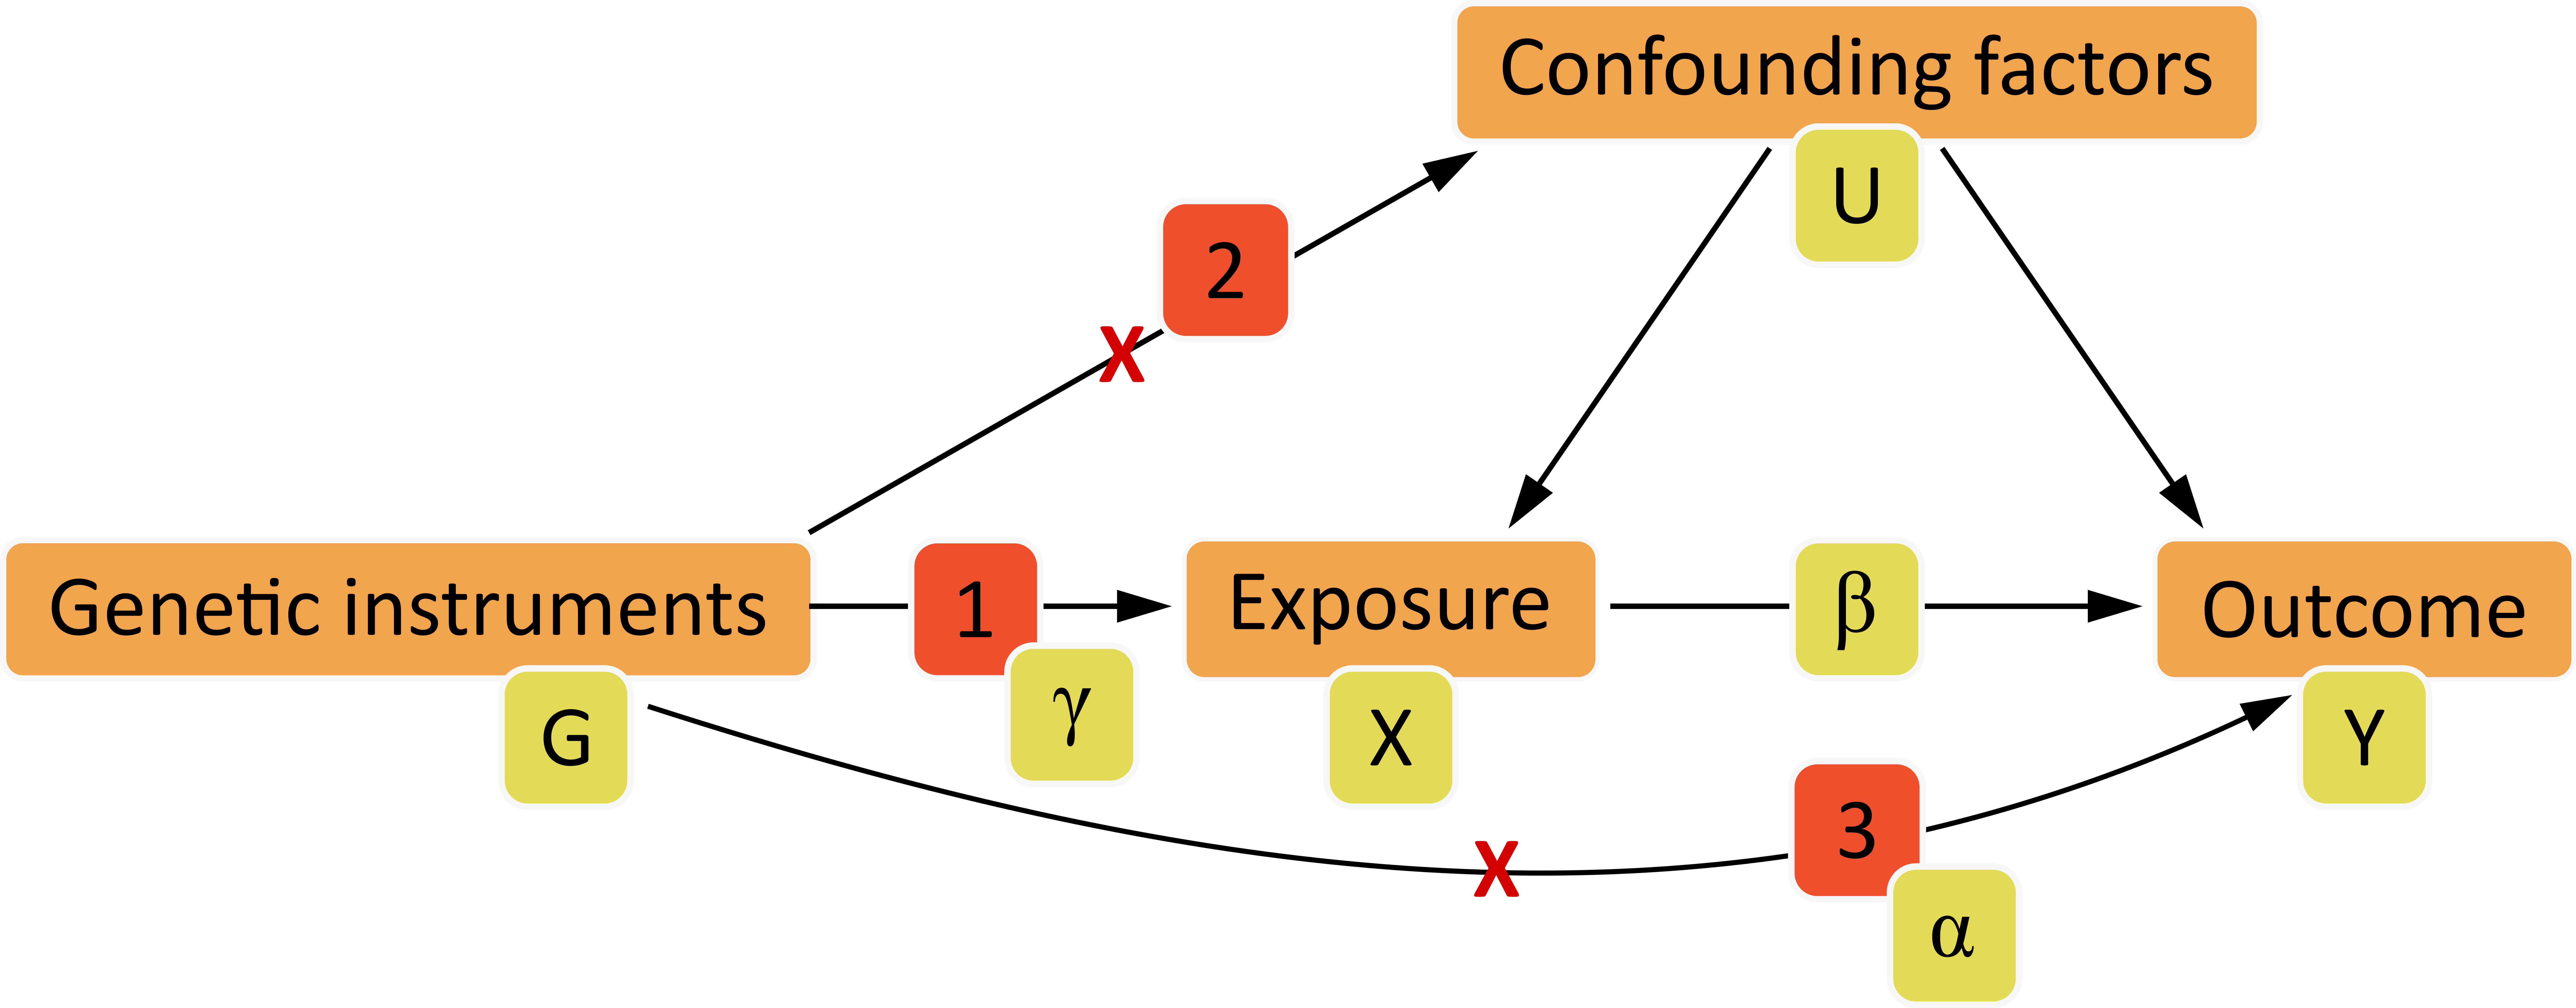
\includegraphics[width=0.5\textwidth,height=\textheight]{C:/Users/sarar/OneDrive/Skrivebord/Virksomhedspraktik/Mendelian-randomization2_figures/MR_analysis_assumptions_w_variables.png}
\caption{A schematic overview of MR analysis and its assumptions
expanded: The yellow boxes indicate the notation given to the assumption
or variable in the statistical methods. \textbf{Assumption 1:} The
instrument is reproducibly and strongly associated with the exposure.
\textbf{Assumption 2:} The instrument is not associated with any known
confounding factors. \textbf{Assumption 3:} The instrument is not
associated with the outcome except through the exposure
(\citeproc{ref-bowden2015}{Bowden, Smith, and Burgess 2015};
\citeproc{ref-sekula2016}{Sekula et al. 2016}).
\label{assumptions_expand}}
\end{figure}

All of the statistical methods start by defining two linear regressions.
One regression of the exposure on the genetic instruments and one of the
outcome on the genetic instruments. This can be done by defining the
following: If:

\begin{itemize}
\tightlist
\item
  \(G_j\) is the jth genetic instrument out of L variables
  \((j=1,...,L)\),
\item
  \(X\) is the exposure,
\item
  \(Y\) is the outcome
\item
  \(U\) is the confounding variables,
\item
  \(\Gamma_j\) is the genetic association with the outcome
\item
  \(\gamma_j\) is the genetic association with the exposure
\item
  \(\beta\) is the causal effect of the exposure on the outcome
\end{itemize}

Then for the \({G_j}^{th}\) instrument the linear regressions are:
\[X_{G_{j}}=\gamma_0+\gamma_jG_j+\varepsilon_{Xj}\tag{1}\]

\[Y_{G_{j}}=\Gamma_0+(\beta\gamma_j+\alpha_j)G_j+\varepsilon_{Yj}=\Gamma_0+\Gamma_jG_j+\varepsilon_{Yj}\tag{2}\]

Since the setting is a two-sample setting the error terms
\(\varepsilon_{Xj}\) and \(\varepsilon_{Yj}\) are independent and it is
assumed that they are normally distributed and contain contributions
from the confounders and all genetic instruments except \(G_j\).
Assumption 1 says that \(\gamma_j\ne 0\) for all \(j\). Assumption 2 and
3 say that the genetic associations with the outcome are equal to the
genetic associations with the exposure multiplied by the causal effect
of the exposure on the outcome:

\[\Gamma_j=\beta\gamma_j+\alpha_j\tag{3}\] Where \(\alpha_j=0\)
(\citeproc{ref-bowden2016}{Bowden et al. 2016})

\(\beta\gamma_j\) is the effect of \(G_j\) on \(Y\) through \(X\), where
we want to estimate \(\beta\) which is the causal effect of \(X\) on
\(Y\) and \(\alpha_j\) represents the association between \(G_j\) and
\(Y\) not through the exposure of interest caused by horizontal
pleiotropy (\citeproc{ref-hartwig2017}{Hartwig, Smith, and Bowden
2017}).

The different methods calculate the estimate of the causal effect of
\(X\) on \(Y\) in different ways.

\subsubsection{\texorpdfstring{\textbf{The Wald
method}}{The Wald method}}\label{the-wald-method}

In the Wald method the slope estimates/regression coefficients from the
two linear regressions, shown above are used to calculate the Wald ratio
(\citeproc{ref-boehm2022}{Boehm and Zhou 2022}):

\[\hat{\beta}_{wald} = \frac{\hat{\Gamma_j}}{\hat{\gamma_j}}\tag{4}\]
This method can be used on GWAS summary statistics however it can only
be used if there is one genetic instrument
(\citeproc{ref-boehm2022}{Boehm and Zhou 2022};
\citeproc{ref-bowden2015}{Bowden, Smith, and Burgess 2015};
\citeproc{ref-sekula2016}{Sekula et al. 2016}).

\subsubsection{\texorpdfstring{\textbf{The Inverse Variance Weighting
Method}}{The Inverse Variance Weighting Method}}\label{the-inverse-variance-weighting-method}

The inverse variance weighting (IVW) method consists of a weighted
linear regression of the genetic associations with the outcome on the
genetic associations with the exposure is performed, this is weighted by
the inverse-variance of the genetic associations with the outcome
\((\sigma_{Yj}^{-2})\). Here the intercept is constrained to equal zero
(\citeproc{ref-bowden2015}{Bowden, Smith, and Burgess 2015}). Each
genetic instrument's effect is weighted by the inverse of the variance
of the ratio estimator. The complete causal effect is then the sum of
the weighted genetic instrument's causal effects
(\citeproc{ref-boehm2022}{Boehm and Zhou 2022}).

\[\hat{\beta}_{IVW} = \frac{\sum_{j}\hat{\gamma_j}^2\sigma_{Yj}^{-2}\hat{\beta_j}}{\sum_{j}\hat{\gamma_j}^2\sigma_{Yj}^{-2}}\tag{5}\]
Since \[\hat\beta_j=\frac{\hat\Gamma_j}{\gamma_j}\tag{6}\] This can also
be written as:
\[\hat{\beta}_{IVW} = \frac{\sum_{j}\hat{\gamma_j}\sigma_{Yj}^{-2}\hat{\Gamma_j}}{\sum_{j}\hat{\gamma_j}^2\sigma_{Yj}^{-2}}\tag{7}\]

This method can be used on several genetic instruments and GWAS summary
statistics (\citeproc{ref-boehm2022}{Boehm and Zhou 2022}). The
breakdown level of IVW is 0\%, meaning that all the genetic instruments
must be valid for the method to provide a consistent estimate
(\citeproc{ref-bowden2016}{Bowden et al. 2016};
\citeproc{ref-hartwig2017}{Hartwig, Smith, and Bowden 2017}). If some of
the genetic instruments are invalid, and directional pleiotropy is
present, the estimates given by IVW suffers from bias and increased Type
1 error rates (\citeproc{ref-bowden2016}{Bowden et al. 2016}).

When the genetic instrument is invalid and \(\alpha\ne0\) the ratio
estimate is then equal to the true causal effect \(\beta\) plus the bias
term \(\frac{\alpha_j}{\gamma_j}\) and therefore IVW will tend toward:

\[\beta+\frac{\sum_{j_1}^{J}\gamma_j\sigma_{Yj}^{-2}\alpha_j}{\sum_{j=1}^{J}\hat{\gamma_j}^2\sigma_{Yj}^{-2}}=\beta+Bias(\alpha,\gamma)\tag{8}\]
(\citeproc{ref-bowden2015}{Bowden, Smith, and Burgess 2015})

\subsubsection{\texorpdfstring{\textbf{The Weighted Median Estimator
Method}}{The Weighted Median Estimator Method}}\label{the-weighted-median-estimator-method}

It is assumed that the genetic variants are uncorrelated, all genetic
instruments are valid, the relationships between the variables are
linear without heterogeneity or effect modification. Remember equations
1-4 and equation 6. Simply put, here the median of all the causal effect
estimates using the genetic instruments is found.

Before attempting the weighted median estimator method it is helpful to
understand the simple median estimator. If \(\hat{\beta}_j\) is the jth
ordered ratio estimate, where all the calculated ratio estimates are
arranged from smallest to largest, and the total number of genetic
instruments are odd \((J=2k+1)\) then the simple median estimator is the
middle ratio estimate \(\hat{\beta}_{k+1}\), where \(k=\frac{J-1}{2}\).
If the total number of genetic instruments is even \(J=2k\) then the
simple median estimator is interpolated between the two middle estimates
\(\frac{1}{2}(\hat{\beta}_{k}+\hat{\beta}_{k+1})\) where
\(k=\frac{J}{2}\). The simple median estimator has a breakdown level of
50\% (exclusively) (\citeproc{ref-bowden2016}{Bowden et al. 2016}).

The simple median estimator is inefficient when the individual estimates
varies a lot. The weighted median estimator accounts for this. \(w_j\)
is the weight given to the jth ordered ratio estimate. The weighted
median estimator is the median of a distribution having estimate
\(\hat{\beta}_j\) as its \(p_j=100(s_j-\frac{w_j}{2})\)th percentile,
where \(s_j\) is the sum of weights up to and including the weight of
the jth ordered estimate \((s_j=\sum_{k=1}^{j}w_k)\). The weights are
standardized so the sum of weights \(s_J\) is 1. The inverse of the
variance of the ratio estimates can be used as weights, giving:
\[w^{'}_j=\frac{\hat{\gamma}^2_j}{\sigma^2_{Y_j}}\tag{9}\] Bowden et
al.~(2016) uses only the first-order term from the delta expansion. The
standardized weights are then
\[w_j=\frac{w_j^{'}}{\sum_jw_j^{'}}\tag{10}\]
(\citeproc{ref-bowden2016}{Bowden et al. 2016}).

The weighted median gives a consistent estimate if at least 50\% of the
weight comes from valid genetic instruments, where it is assumed that no
single genetic instrument contributes more than 50\% of the weight, so
it has a breakdown level of 50\% (exclusively)
(\citeproc{ref-bowden2016}{Bowden et al. 2016}).

\subsubsection{\texorpdfstring{\textbf{The MR-Egger Regression
Method}}{The MR-Egger Regression Method}}\label{the-mr-egger-regression-method}

The weighted linear regression is performed without the intercept being
constrained to zero. Here the intercept represents the average
pleiotropic effect across the genetic instruments. The MR-Egger test,
then consists of assessing whether or not the intercept differs from
zero. If this is the case it indicates the presence of directional
pleiotropy. If the InSIDE assumption is satisfied the slope coefficient
from the MR-egger regression is a consistent estimate of the causal
effect. The InSIDE assumption is violated if the pleiotropic effects act
through a confounder of the exposure (\citeproc{ref-bowden2015}{Bowden,
Smith, and Burgess 2015}).

If a genetic instrument is not valid because it has a direct effect on
the outcome (assumption 3 is not satisfied), then \(\alpha\ne0\) and the
ratio estimate based on the genetic instrument j is (in an infinite
sample) then equal to the true causal effect \(\beta\) plus the bias
term \(\frac{\alpha_j}{\gamma_j}\):
\[\beta_j=\beta+\frac{\alpha_j}{\gamma_j}\tag{11}\]

The IVW estimate is the slope of the best fitting lines through the data
points, that also passes through the origin. When the InSIDE assumption
is satisfied, \(\hat\alpha_j\) is independent of \(\hat\gamma_j\),
therefore the bias of the ratio estimate
\(\hat\beta_j=\frac{\hat\Gamma_j}{\hat\gamma_j}\) is inversely
proportional to \(\gamma_j\)

When regression of the \(\hat\Gamma_j\) coefficients on the
\(\hat\gamma_j\) and the intercept is not constrained to zero the
following linear model is found/made, which performs Egger regression:
\[\hat\Gamma_j=\beta_{0E}+\beta_E\hat\gamma_j\tag{12}\] If the intercept
term \((\beta_{0E})\) is not zero it indicates the presence of
directional pleiotroy (this is the Egger's test), therefore the
estimated value of \((\beta_{0E})\) can be used as an estimate of the
average pleiotropic effect. \(\hat\beta_E\) is a bias-reduced estimate,
since (under model 12) the following is true for the slope coefficient
from Egger regression:
\[\hat\beta_E=\frac{cov(\hat\Gamma,\hat\gamma)}{var(\hat\gamma)}=\hat\beta+\frac{cov(\hat\alpha,\hat\gamma)}{var(\hat\gamma)}\tag{13}\]
Because of the InSIDE assumption the following is then true:
\[cov(\hat\alpha,\hat\gamma)\xrightarrow{N\to\infty}cov(\alpha,\gamma)\xrightarrow{J\to\infty}0\tag{14}\]
Meaning that \(\hat\beta_E\) is a consistent estimate of \(\beta\) (the
causal effect) (\citeproc{ref-bowden2015}{Bowden, Smith, and Burgess
2015}).

If the InSIDE assumption is satisfied the breakdown level of the
MR-Egger method is 100\% (\citeproc{ref-bowden2016}{Bowden et al. 2016};
\citeproc{ref-hartwig2017}{Hartwig, Smith, and Bowden 2017}). However
the MR-Egger often has low statistical power for effect estimation, and
it has been suggested that it should primarily be used to reveal
pleiotropy, as a sensitivity analysis, in addition to the other methods
(\citeproc{ref-haycock2016}{Haycock et al. 2016};
\citeproc{ref-burgess2017}{Burgess and Thompson 2017}).

\subsubsection{\texorpdfstring{\textbf{The Simple Mode and Weighted Mode
Method}}{The Simple Mode and Weighted Mode Method}}\label{the-simple-mode-and-weighted-mode-method}

When calculating the mode-based estimate, the mode of the smoothed
empirical density function of all \(\hat\beta_j\)s is used as the causal
effect estimate, but before doing this a few things must be defined.

It is assumed that all L genetic variants are independent of each other.

Remember \(\beta\gamma_j\) is the effect of G\textsubscript{j} on Y
through X, where we want to estimate \(\beta\) which is the causal
effect of X on Y and \(\alpha_j\) represents the association between
G\textsubscript{j} and Y not through the exposure of interest caused by
horizontal pleiotropy.

When \(\alpha_j\ne0\) then \(\hat\beta_j=\beta+b_j\) where
\(b_j=\frac{\alpha_j}{\gamma_j}\) also called the bias term. For the
simple mode and weighted mode to consistently estimate the true causal
effect, the ZEMPA assumption must be satisfied, which says that across
all the instruments, the most frequent value (the mode) of \(b_j\) is 0
(\citeproc{ref-hartwig2017}{Hartwig, Smith, and Bowden 2017}).

If \(k\in\{1,2,...,L\}\) represents the number of unique values of
\(b_j\) among L variants, then if all \(b_j\) terms are identical then
\(k=1\), but if they are all unique then \(k=L\). Additionally
\(n_1,n_2,...,n_k\) represents the number of genetic instruments that
have identical non-zero value of \(b_j\), \(n_1\) having the smallest
non-zero value and \(n_k\) having the largest non-zero value, \(n_0\) is
then the number of genetic instruments with \(b_j=0\) and these are the
valid instruments. The number of variants is then:
\[L=n_0+n_1+n_2+...+n_k\tag{15}\] When ZEMPA is satisfied, the following
must then be true: \[n_0>\max(n_1,...,n_k)\tag{16}\] Meaning that the
number of valid genetic instruments is larger than any other group of
genetic instruments with the same bias term
(\citeproc{ref-hartwig2017}{Hartwig, Smith, and Bowden 2017}).

The breakdown level of the simple mode method ranges from:
\[100\left(\frac{\frac{L}{2}+1}{L}\right)\%\text{ to }100\left(\frac{L-2}{L}\right)\tag{17}\]
Where the lower limit is the situation where there are some valid
genetic instruments, but all the invalid genetic instruments estimate
the same causal effect parameter - they all have the same bias term,
meaning that the ZEMPA assumption is satisfied when up to, but not
including, half of the instruments are invalid. The upper limit is the
situation where all invalid instruments have different bias terms, so
they estimate different causal effect parameters
\((n_1=n_2=...=n_k=1)\). Here ZEMPA is satisfied if only two of the
genetic instruments are valid and the remainder invalid. When the larges
number of identical estimates comes from invalid instruments ZEMPA is
violated (\citeproc{ref-hartwig2017}{Hartwig, Smith, and Bowden 2017}).

In the weighted mode method ZEMPA is satisfied if the weights associated
with the valid genetic instruments are the largest among all \(k\)
subsets of instruments, giving: \[w_0>max(w_1,...,w_k)\tag{18}\]

The breakdown level of the weighted mode method ranges from 50\%
(exclusive) to 100\% (exclusive). As the number of genetic instruments
increases the lower and upper limits of the breakdown level tend toward
50\% and 100\% (\citeproc{ref-hartwig2017}{Hartwig, Smith, and Bowden
2017}).

As mentioned in the beginning of this section the mode of the smoothed
empirical density function of all \(\hat\beta_j\)s is used as the causal
effect estimate. The standardized weights for the weighted mode estimate
can be found using:
\[w_j=\frac{\sigma_{Rj}^{-2}}{\sum_{j=1}^{L}\sigma_{Rj}^{-2}}\tag{19}\]
Where \(\sigma_{Rj}^{-2}\) is the standard error of \(\hat\beta_j\) and
can be calculated by:

\[\sigma_{Rj}=\sqrt{\frac{\sigma_{Yj}^{2}}{\hat\gamma_j^2}+\frac{\hat\Gamma_j^2\sigma_{Xj}^{2}}{\hat\gamma_j^4}}\tag{20}\]
For the simple mode estimate \(w_1=w_2=...=w_L=1/L\)

The normal kernel density function of the \(\hat\beta_j\)s is:

\[f(x)=\frac{1}{h\sqrt{2\pi}}\sum_{j=1}^{L}w_j\exp\left[-\frac{1}{2}\left(\frac{x-\hat\beta_j}{h}\right)^2\right]\tag{21}\]
\(h\) is the smoothing bandwidth parameter and it regulates a
bias-variance trade-off of the mode-based method, meaning that higher
\(h\) leads to higher precision and higher bias. \(h\) can be found by:
\[h=\phi s\tag{22}\] \(\phi\) is a tuning parameter which allow
increased or decreased bandwidth. \(s\) is the default bandwidth chosen
according to a criteria. Hartwig, Smith, and Bowden
(\citeproc{ref-hartwig2017}{2017}) uses the modified Silverman's
bandwidth rule:
\[s=\frac{0.9\min(sd(\hat\beta_j),1.4826mad(\hat\beta_j))}{L\frac{1}{5}}\tag{23}\]
Here \(sd(\hat\beta_j)\) is the standard deviation and
\(mad(\hat\beta_j)\) is the median absolute deviation from the
\(L\hat\beta_j\)s.

The causal effect estimate obtained using this method \((\hat\beta_M)\)
is the value of \(x\) that maximizes \(f(x)\)
\(\left(f\left(\hat\beta_M\right)=\max[f(x)]\right)\)
(\citeproc{ref-hartwig2017}{Hartwig, Smith, and Bowden 2017}).

This theoretical and mathematical background is useful when performing
the MR analysis, since it helps when choosing which method to use.
However several of the methods can be performed at once and the results
compared to see if they ``agree'', but it is important to remember the
assumptions behind the methods and discuss if they are met, since all
the methods may produce an estimate, but not all may be reliable in your
situation.

\subsection{Interpreting and understanding MR analysis results in
research
articles}\label{interpreting-and-understanding-mr-analysis-results-in-research-articles}

One thing is understanding the mechanics behind the MR studies, another
thing is understanding how research articles present the results from
their MR analyses. This section will try to provide some insight into
this.

The first thing to remember is that all of the methods give an estimate
of \(\beta\). If this estimate is significant and positive it indicates
that there is a causal relationship between the exposure and the
outcome.

A scatter plot can be presented, with all the genetic instruments
(SNPs), where the genetic instrument-outcome association is on the
Y-axis and the genetic instrument-exposure association is on the X-axis.
In the plot the 95\% confidence interval for the exposure and outcome
association, for each genetic instrument is also shown as horizontal and
vertical lines from each data point representing a genetic instrument.
For the IVW method a line is then added which joins the data points to
the origin. In this way the plot visualizes the used genetic instruments
and it may reveal if some of the genetic instruments perhaps are be
outliers. If outliers are present, it may affect the estimated \(\beta\)
value given by the different methods, where the MR-Egger method is more
influenced by outliers than the simple mode and weighted mode
(\citeproc{ref-bowden2019}{Bowden and Holmes 2019};
\citeproc{ref-burgess2017}{Burgess and Thompson 2017}). If a line
representing the MR-Egger regression is included in the scatter plot,
this can be used to see if directional pleiotropy is present in the
data. However the InSIDE assumption must be met for this sensitivity
analysis to hold. If the InSIDE assumption is satisfied and the
intercept of MR-Egger regression differs from zero it could indicate the
presence of directional pleiotropy (\citeproc{ref-bowden2019}{Bowden and
Holmes 2019}). In Figure \ref{scatterplot_example} an example of such a
scatter plot can be seen, the scatter plot is from Bowden and Holmes
(\citeproc{ref-bowden2019}{2019}).

\begin{figure}
\centering
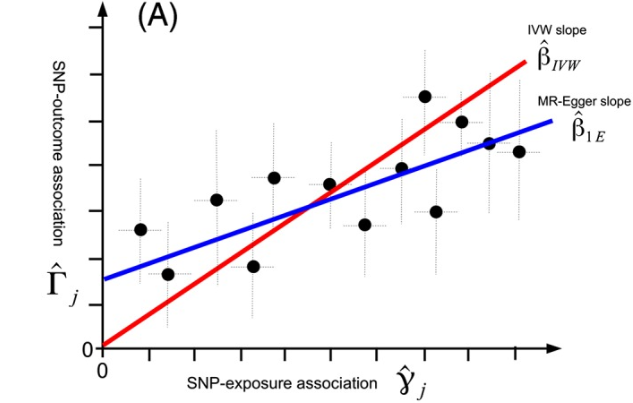
\includegraphics[width=0.5\textwidth,height=\textheight]{C:/Users/sarar/OneDrive/Dokumenter/R/bowden2019_fig4a.png}
\caption{An example of a scatter plot where the data point for the
genetic instruments are plotted according to their association with the
exposure and outcome, the 95\% confidence intervals for these
associations are also shown with the horizontal and vertical lines
protruding from each data point. The lines represent the ratio estimate
found using either the IVW method or the MR-Egger method. The figure is
from Bowden and Holmes (\citeproc{ref-bowden2019}{2019}).
\label{scatterplot_example}}
\end{figure}

A funnel plot can also be presented with the data points from each
individual genetic instrument, where the causal effect estimates are on
the X-axis and the square-root precision is on the Y-axis. The funnel
plot will be symmetrical if there is either no pleiotropy or balanced
pleiotropy. If the InSIDE assumption holds the MR-Egger estimate in an
asymmetrical funnel plot can then be interpreted as the value that a
symmetrical would have produced (\citeproc{ref-bowden2019}{Bowden and
Holmes 2019}). An example of such a funnel plot can be seen in Figure
\ref{funnelplot_example}, the funnel plot is from Bowden and Holmes
(\citeproc{ref-bowden2019}{2019}).

\begin{figure}
\centering
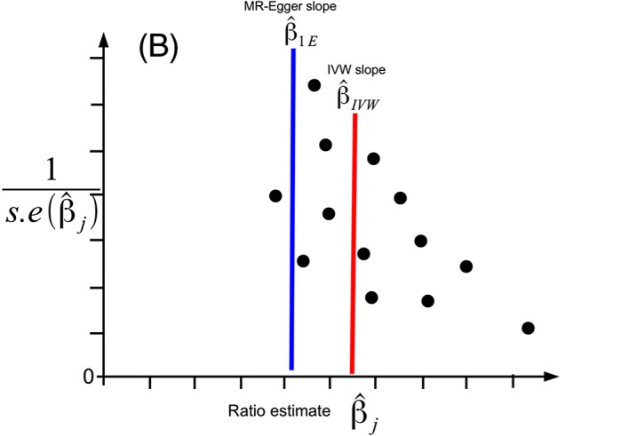
\includegraphics[width=0.5\textwidth,height=\textheight]{C:/Users/sarar/OneDrive/Dokumenter/R/bowden2019_fig4b.png}
\caption{An example of a funnel plot where the data point for the
genetic instruments are plotted according to their causal effect
estimates and the square-root precision. Since the funnel plot is not
symmetrical it indicates the presence of directional pleiotropy. The
figure is from Bowden and Holmes
(\citeproc{ref-bowden2019}{2019}).\label{funnelplot_example}}
\end{figure}

Additionally Q and Q' statistics can also be shown, which can also help
interpreting the likelihood of statistical heterogeneity around the IVW
and MR-Egger estimates due to horizontal pleiotropy, especially if the
Q-Q' difference is great. If this is the case it may be relevant to
check if an outlier analysis has been performed, to examine if one
genetic instrument drives the heterogeneity
(\citeproc{ref-bowden2019}{Bowden and Holmes 2019}).

Some papers also present a forest plot like the ones seen in
meta-analyses, either over the combined odds ratio from the different
methods they have used, or showing all the odds ratios (Wald ratios)
from the genetic instruments used. The last type of forest plot, may be
a result of a leave-one-out analysis, or just to show the individual
Wald ratios.

The paper by Davies, Holmes, and Smith (\citeproc{ref-davies2018}{2018})
also explains how to be critical of results from MR studies and provides
a list of questions one can ask oneself when reading research papers
concerning MR studies.

\subsection{Using the Two Sample MR analysis
package}\label{using-the-two-sample-mr-analysis-package}

The package MRCIEU/TwoSampleMR can be used to perform an MR analysis
(\citeproc{ref-twosamplemr}{Hemani et al. 2018};
\citeproc{ref-mrsteiger}{Hemani, Tilling, and Davey Smith 2017};
\citeproc{ref-intro}{Hermani, n.d.c}). This is done in four steps:

\begin{enumerate}
\def\labelenumi{\arabic{enumi}.}
\tightlist
\item
  Selecting the instruments for the exposure
\item
  Acquiring the instruments from the IEU GWAS database for the outcome
\item
  Harmonizing the effect sizes for the instruments on the exposure and
  outcomes to be for the same reference allele.
\item
  Performing the MR analysis (\citeproc{ref-twosamplemr}{Hemani et al.
  2018}; \citeproc{ref-mrsteiger}{Hemani, Tilling, and Davey Smith
  2017}; \citeproc{ref-intro}{Hermani, n.d.c}).
\end{enumerate}

\subsubsection{Selecting the instruments for the
exposure}\label{selecting-the-instruments-for-the-exposure}

The R commands used in this step are:

\begin{itemize}
\tightlist
\item
  \texttt{extract\_instruments()}
\item
  \texttt{read\_exposure\ data()}
\item
  \texttt{library(MRInstruments)}

  \begin{itemize}
  \tightlist
  \item
    \texttt{data(gwas\_catalog)}
  \item
    \texttt{data(aries\_mqtl)}
  \item
    \texttt{data(gtex\_eqtl)}
  \item
    \texttt{data(proteomic\_qtls)}
  \item
    \texttt{data(metab\_qtls)}
  \end{itemize}
\item
  \texttt{clump\_data()}
\end{itemize}

To perform the analysis this package need the information concerning the
instruments in a data frame, where each line has the information for one
variant for one exposure. Different types information concerning the
instrument is needed as seen in the table below.

\begin{longtable}[]{@{}
  >{\raggedright\arraybackslash}p{(\columnwidth - 2\tabcolsep) * \real{0.7703}}
  >{\raggedright\arraybackslash}p{(\columnwidth - 2\tabcolsep) * \real{0.2297}}@{}}
\caption{An overview of the information that can be used in the
two-sample mendelian analysis. *This information is necessary for the
analysis.}\tabularnewline
\toprule\noalign{}
\begin{minipage}[b]{\linewidth}\raggedright
Type of information
\end{minipage} & \begin{minipage}[b]{\linewidth}\raggedright
name/label
\end{minipage} \\
\midrule\noalign{}
\endfirsthead
\toprule\noalign{}
\begin{minipage}[b]{\linewidth}\raggedright
Type of information
\end{minipage} & \begin{minipage}[b]{\linewidth}\raggedright
name/label
\end{minipage} \\
\midrule\noalign{}
\endhead
\bottomrule\noalign{}
\endlastfoot
The rs ID* & \texttt{SNP} \\
The effect size (is the trait binary, use log(OR))* & \texttt{beta} \\
The standard error of the effect size* & \texttt{se} \\
The allele of the SNP which has the effect \texttt{beta}* &
\texttt{effect\_allele} \\
The non-effect allele & \texttt{other\_allele} \\
The effect allele frequency & \texttt{eaf} \\
The name of the phenotype the SNP has an effect on &
\texttt{phenotype} \\
Physical position of the variant (chromosome) & \texttt{chr} \\
Physical position of variant (position) & \texttt{position} \\
Sample size for estimating the effect size & \texttt{samplesize} \\
The number of cases & \texttt{ncase} \\
The number of controls & \texttt{ncontrol} \\
The P-value for the SNP's association with the exposure &
\texttt{pval} \\
The units in which the effects are presented & \texttt{units} \\
The gene or other annotation for the SNP & \texttt{gene} \\
\end{longtable}

This information/exposure data can either be acquired from a text file
using the \texttt{read\_exposure\_data} function, where the file has a
header with column names according to the labels in the table above. If
the text file does not have column names according to the labels in the
table above, they must be defined, so the data is read correctly. This
can be done in the \texttt{read\_exposure\_data}:

\begin{Shaded}
\begin{Highlighting}[]
\CommentTok{\#library(TwoSampleMR)}
\CommentTok{\#name\_of\_file \textless{}{-} system.file("place of file")}
\CommentTok{\#exposure\_phenotype\_exp\_dat \textless{}{-} read\_exposure\_data(}
\CommentTok{\#     filename = name\_of\_file,}
\CommentTok{\#     sep = ",", \#if it is a comma seperating the fields}
\CommentTok{\#     snp\_col = "name of snp column in file"}
\CommentTok{\#     beta\_col = "name of effect size column in file"}
\CommentTok{\#     se\_col = "name of se column in file"}
\CommentTok{\#     effect\_allele\_col = "name of effect allele column in file"}
\CommentTok{\#     other\_allele\_col = "name of non{-}effect allele column in file"}
\CommentTok{\#     eaf\_col = "name of effect allele frequency column in file"}
\CommentTok{\#     pval = "name of the pval column in file"}
\CommentTok{\#     units\_col = "name of the units column in file"}
\CommentTok{\#     gene\_col = "name of the gene column in file"}
\CommentTok{\#     samplesize\_col = "name of the sample size column in file"}
\CommentTok{\#)}
\end{Highlighting}
\end{Shaded}

In case the \texttt{phenotype} column is not in the imported file, is
will be assumed that the phenotype's name is ``exposure'', which is
entered in the exposure column, but it can be renamed by

\begin{Shaded}
\begin{Highlighting}[]
\CommentTok{\#exposure\_phenotype\_exp\_dat$exposure \textless{}{-} "phenotype"}
\end{Highlighting}
\end{Shaded}

If data is acquired from a previous file, the
\texttt{read\_exposure\_data} converts the data to a data frame with
standardized column names

The exposure data can also be acquired from a previous data frame, the
\texttt{format\_data()} function will convert the data to the correct
format.

GWAS databases can also be browsed for instruments through the
\texttt{MRInstruments} package. The GWAS catalog can be found/browsed
the following way:

\begin{Shaded}
\begin{Highlighting}[]
\CommentTok{\#library(TwoSampleMR)}
\CommentTok{\#library(MRInstruments)}
\CommentTok{\#data(gwas\_catalog)}
\CommentTok{\#head(gwas\_catalog)}
\end{Highlighting}
\end{Shaded}

A list of studies is then shown. A study can then be chosen from which
the instruments will be found and the data defined in a variable named
\texttt{exposure\_phenotype\_exp\_dat} as shown below:

\begin{Shaded}
\begin{Highlighting}[]
\CommentTok{\#exposure\_phenotype\_gwas \textless{}{-}}
\CommentTok{\#   subset(gwas\_catalog,}
\CommentTok{\#          grepl("Authorname", Author) \&}
\CommentTok{\#            Phenotype == "exposure\_phenotype") }
\CommentTok{\#exposure\_phenotype\_exp\_dat \textless{}{-} format\_data(exposure\_phenotype\_gwas)}
\end{Highlighting}
\end{Shaded}

The IEU GWAS database can also be accessed to define instruments for an
exposure.

When the data has been acquired it is important to ensure that the
instruments (for exposure) are independent. This can be done using the
\texttt{clump\_data()} function.

\begin{Shaded}
\begin{Highlighting}[]
\CommentTok{\#exposure\_phenotype\_dat \textless{}{-} clumping\_data(exposure\_phenotype\_exp\_data\_from\_study}
\CommentTok{\#str(exposure\_phenotype\_dat))}
\end{Highlighting}
\end{Shaded}

\emph{A more thorough review of this step can be found
\href{https://mrcieu.github.io/TwoSampleMR/articles/exposure.html}{here.}}
(\citeproc{ref-twosamplemr}{Hemani et al. 2018};
\citeproc{ref-mrsteiger}{Hemani, Tilling, and Davey Smith 2017};
\citeproc{ref-expdat}{Hermani, n.d.a})

\subsubsection{Acquiring the instruments from the IEU GWAS database for
the
outcome}\label{acquiring-the-instruments-from-the-ieu-gwas-database-for-the-outcome}

The R commands used in this step are:

\begin{itemize}
\tightlist
\item
  \texttt{extract\_outcome\_data()}
\item
  \texttt{read\_outcome\_data()}
\item
  (\texttt{available\_outcomes()})
\end{itemize}

Now the instruments associated with the exposure trait has been
identified. The next step is to extract these genetic variants from the
outcome data. Remember that we are looking for the same genetic
instruments as we have just found, but now associated with the outcome,
and from a different study population.

Here the IEU GWAS database can be browsed again. Details about the
available GWASs can be found the following way:

\begin{Shaded}
\begin{Highlighting}[]
\CommentTok{\#library(TwoSampleMR)}
\CommentTok{\#ao \textless{}{-} available\_outcomes()}
\CommentTok{\#head(ao)}
\end{Highlighting}
\end{Shaded}

The \texttt{available\_outcomes()} function gives a table of the
available studies (each with a unique ID) in the database. The ID of the
study is used, when extracting SNPs from a specific study the following
way:

\begin{Shaded}
\begin{Highlighting}[]
\CommentTok{\#exposure\_phenotype\_exp\_dat \textless{}{-} extract\_instruments(outcomes = "study ID")}
\CommentTok{\#head(exposure\_phenotype\_exp\_dat)}
\end{Highlighting}
\end{Shaded}

\begin{Shaded}
\begin{Highlighting}[]
\CommentTok{\#ao[grepl("outcome trait", ao$trait), ]}
\end{Highlighting}
\end{Shaded}

This gives a list of possible GWAS studies, the wanted SNPs from the
selected study can then be acquired by:

\begin{Shaded}
\begin{Highlighting}[]
\CommentTok{\#outcome\_phenotype\_out\_dat \textless{}{-} extract\_outcome\_data(}
\CommentTok{\#    snps = exposure\_phenotype\_exp\_dat$SNP,}
\CommentTok{\#    outcomes = \textquotesingle{}study ID\textquotesingle{}}
\CommentTok{\#)}
\end{Highlighting}
\end{Shaded}

In \texttt{the\ extract\_outcome\_data()} function the \texttt{snps}
argument only require an array of rsIDs and the \texttt{outcomes}
argument can be a vector of outcomes.

If a specifically requested SNP is not present in the outcome GWAS then
a SNP (proxy) that is in linkage disequilibrium with the requested SNP
(target) is searched for instead.

Local GWAS summary data can also be used

\emph{A more thorough review of this step can be found
\href{https://mrcieu.github.io/TwoSampleMR/articles/outcome.html}{here.}}
(\citeproc{ref-twosamplemr}{Hemani et al. 2018};
\citeproc{ref-mrsteiger}{Hemani, Tilling, and Davey Smith 2017};
\citeproc{ref-outdat}{Hermani, n.d.d})

\subsubsection{Harmonizing the exposure and outcome
data}\label{harmonizing-the-exposure-and-outcome-data}

The R commands used in this step are:

\begin{itemize}
\tightlist
\item
  \texttt{harmonise\_data()}
\item
  \texttt{power\_prune()}
\end{itemize}

Now you have both the exposure and outcome data saved in the two
variables \texttt{exposure\_phenotype\_exp\_dat} and
\texttt{outcome\_phenotype\_out\_dat}.The next step is to harmonize the
effect of a SNP on the exposure and the effect of that SNP on the
outcome, so they correspond to the same allele. This is done the
following way:

\begin{Shaded}
\begin{Highlighting}[]
\CommentTok{\#library(TwoSampleMR)}
\CommentTok{\#dat \textless{}{-} harmonise\_data (}
\CommentTok{\#  exposure\_dat = exposure\_phenotype\_exp\_dat,}
\CommentTok{\#  outcome\_dat = outcome\_phenotype\_out\_dat}
\CommentTok{\#)}
\end{Highlighting}
\end{Shaded}

The output is a new data frame where the exposure and outcome data is
combined.

There three ways to harmonize data:

\begin{enumerate}
\def\labelenumi{\arabic{enumi}.}
\tightlist
\item
  Assume that all alleles are presented on the forward strand.
\item
  Try to infer the forward stand alleles using allele frequency
  information.
\item
  Correct the strand for non-palindromic SNPs, but drop palindromic
  SNPs.
\end{enumerate}

The \texttt{harmonise\_data} function uses option 2 as a default, but by
using the \texttt{action} argument, this can be modified:
\texttt{harmonise\_data(exposure\_dat,\ outcome\_dat,\ action\ =\ 3)}

The dataset may contain duplicate exposure-outcome summary sets after
data harmonisation. It is recommended that duplicate exposure-outcome
summary sets are removed, so only the exposure-outcome combination with
the highest expected power remains, this can be done using the
\texttt{power\_prune()} function.

\begin{Shaded}
\begin{Highlighting}[]
\CommentTok{\# dat \textless{}{-} power\_prune(dat, method = 1, dist.outcome = "binary")}
\end{Highlighting}
\end{Shaded}

The method can be set to either 1 or 2. When the method is set to 1, the
duplicate exposure-outcome sets with the smaller outcome sample size are
removed. If there are still duplicates, they are removed according to
the exposure sample size. If there are many SNPs available to instrument
an exposure, the outcome GWAS with the better SNP coverage might have
better power than the outcome GWAS with the larger sample size. In this
case the method is set to 2. The studies are the removed according to
instrument strength as well as sample size. Here it is assumed that the
SNP-exposure effects correspond to a continuous trait with a normal
distribution. If the exposure is binary then the method should be set to
1.

\emph{A more thorough review of this step can be found
\href{https://mrcieu.github.io/TwoSampleMR/articles/harmonise.html}{here.}}
(\citeproc{ref-twosamplemr}{Hemani et al. 2018};
\citeproc{ref-mrsteiger}{Hemani, Tilling, and Davey Smith 2017};
\citeproc{ref-harmdat}{Hermani, n.d.b})

\subsubsection{Performing the MR
analysis}\label{performing-the-mr-analysis}

The R commands used in this step are:

\begin{itemize}
\tightlist
\item
  \texttt{mr()}
\item
  \texttt{mr\_singlesnp()}
\item
  \texttt{leaveoneout()}
\item
  \texttt{mr\_heterogeneity()}
\item
  \texttt{mr\_steiger()}
\item
  \texttt{mr\_pleiotropy\_test()}
\end{itemize}

When we have acquired the exposure data and the outcome data and this
has been harmonized the MR analysis can be performed, since the effects
and standard errors for each instrument SNP present/available for the
exposure and outcome traits has now been acquired. The MR analysis is
performed using the \texttt{mr()} function.

\begin{Shaded}
\begin{Highlighting}[]
\CommentTok{\#library(TwoSampleMR)}
\CommentTok{\#library(ggplot2)}
\CommentTok{\#res \textless{}{-} mr(dat)}
\end{Highlighting}
\end{Shaded}

The output is a data frame where the causal effect of the exposure on
the outcome is calculated using five different MR methods (MR Egger,
Weighted median, Inverse variance weighted, Simple mode, Weighted mode).
If only some of these MR methods should be performed, they can be
specified the following way:

\begin{Shaded}
\begin{Highlighting}[]
\CommentTok{\#mr(dat, method\_list = c("wanted MR analysis1", "wanted MR analysis2))}
\end{Highlighting}
\end{Shaded}

The name of the wanted analysis that should be specified can be found
using the \texttt{mr\_method\_list} function, which yields a long list
of MR methods and their given names in the package.

A heterogeneity test can be performed using the
\texttt{mr\_heterogeneity()} function, here that should be used can also
be specified.

A horizontal pleiotropy test, where the intercept term in the MR Egger
regression is used, can also be performed using the
\texttt{mr\_pleiotropy\_test()} function.

If several MR estimates using each of the SNPs is desired the
\texttt{mr\_singlesnp()} function can be used. The output of this
function is a data frame where the MR analysis has been performed
several times for each exposure-outcome combination, where a different
single SNP has been used every time. The Wald ratio is used to perform
the analysis, but if the fixed effects meta analysis method should be
used instead, it can be specified the following way:

\begin{Shaded}
\begin{Highlighting}[]
\CommentTok{\#res\_single \textless{}{-} mr\_singlesnp(dat, single\_method = "mr\_meta\_fixed")}
\end{Highlighting}
\end{Shaded}

The \texttt{mr\_singlesnp()} function also calculates the full MR using
all available SNPs using IVW and MR Egger. It can be specified the
following way:

\begin{Shaded}
\begin{Highlighting}[]
\CommentTok{\#res\_single \textless{}{-} mr\_singlesnp(dat, all\_method = "mr\_two\_sample\_ml")}
\end{Highlighting}
\end{Shaded}

Then only the maximum likelihood method for the combined test is
performed. The \texttt{mr\_singlesnp()} function needs to be performed
if a forest plot that compares the MR estimates using the different MR
methods against the single SNP tests is desired.

To identify if a single SNP is driving the association a leave-one-out
analysis can be performed, where the MR is performed leaving out each
SNP in turn. To do this use the \texttt{mr\_leaveoneout()} function:

\begin{Shaded}
\begin{Highlighting}[]
\CommentTok{\#res\_loo \textless{}{-} mr\_leaveoneout(dat)}
\end{Highlighting}
\end{Shaded}

The default method is IVW, but the method argument can be used to change
this.

\emph{A more thorough review of this step can be found
\href{https://mrcieu.github.io/TwoSampleMR/articles/perform_mr.html}{here.}}
(\citeproc{ref-twosamplemr}{Hemani et al. 2018};
\citeproc{ref-mrsteiger}{Hemani, Tilling, and Davey Smith 2017};
\citeproc{ref-MR}{Hermani, n.d.e})

\paragraph{\texorpdfstring{\textbf{Visualizing the
results:}}{Visualizing the results:}}\label{visualizing-the-results}

\emph{A more thorough review of this step and the different plots can be
found
\href{https://mrcieu.github.io/TwoSampleMR/articles/perform_mr.html}{here.}}
(\citeproc{ref-twosamplemr}{Hemani et al. 2018};
\citeproc{ref-mrsteiger}{Hemani, Tilling, and Davey Smith 2017};
\citeproc{ref-MR}{Hermani, n.d.e})

\paragraph{Scatter plot}\label{scatter-plot}

A scatter plot that depicts the relationship of the SNP effects on the
exposure against the SNP effects on the outcome can be made using the
\texttt{mr\_scatter\_plot()} function:

\begin{Shaded}
\begin{Highlighting}[]
\CommentTok{\#library(TwoSampleMR)}
\CommentTok{\#library(ggplot2)}
\CommentTok{\#res \textless{}{-} mr(dat)}
\CommentTok{\#p1 \textless{}{-} mr\_scatter\_plot(res, dat)}
\end{Highlighting}
\end{Shaded}

This creates a scatter plot for each exposure-outcome test, stored in
\texttt{p1} To plot the first plot write:

\begin{Shaded}
\begin{Highlighting}[]
\CommentTok{\#p1[[1]]}
\end{Highlighting}
\end{Shaded}

To see the number of plots stored in p1 use the \texttt{length()}
function:

\begin{Shaded}
\begin{Highlighting}[]
\CommentTok{\#length(p1)}
\end{Highlighting}
\end{Shaded}

For each method used in \texttt{mr(dat)} a line is drawn corresponding
to the estimated causal effect. To limit the number of lines, the
desired methods can be defined in the \texttt{mr(dat)} function as shown
above.

The plot can be saved as either a pdf or png using \texttt{ggsave()}:

\begin{Shaded}
\begin{Highlighting}[]
\CommentTok{\#ggsave(p1[[1]], file = "filename.pdf", width = 8, height = 8)}
\CommentTok{\#OR}
\CommentTok{\#ggsave(p1[[1]], file = "filename.png", width = 8, height = 8)}
\end{Highlighting}
\end{Shaded}

\paragraph{Forest Plot}\label{forest-plot}

To create a forest plot that compares the MR estimates using the
different MR methods against the single SNP tests, the
\texttt{mr\_forest\_plot()} function can be used:

\begin{Shaded}
\begin{Highlighting}[]
\CommentTok{\#p2 \textless{}{-} mr\_forest\_plot(res\_single)}
\CommentTok{\#p2[[1]]}
\end{Highlighting}
\end{Shaded}

The plot shows the causal effects as estimated using each of the SNPs on
their own and compared against the causal effect as estimated using the
methods that use alle the SNPs. If different methods are desired in the
plot, they should be specified in the \texttt{mr\_singlesnp()} function.

\paragraph{Leave-one-out plot}\label{leave-one-out-plot}

The \texttt{mr\_leaveoneout\_plot()} can be used to visualize the
leave-one-out analysis:

\begin{Shaded}
\begin{Highlighting}[]
\CommentTok{\#p3 \textless{}{-} mr\_leaveoneout\_plot(res\_loo)}
\CommentTok{\#p3[[1]]}
\end{Highlighting}
\end{Shaded}

If a specific MR analysis is desired it can be specified in the
\texttt{mr\_leaveoneout()} function using
\texttt{method\ =\ "name\ of\ MR\ analysis"}

\paragraph{Funnel plot:}\label{funnel-plot}

A funnel plot can be made using the single SNP results from the
\texttt{mr\_singlesnp()} function by using the
\texttt{mr\_funnel\_plot()} function:

\begin{Shaded}
\begin{Highlighting}[]
\CommentTok{\#p4 \textless{}{-} mr\_funnel\_plot(res\_single)}
\CommentTok{\#p4[[1]]}
\end{Highlighting}
\end{Shaded}

\paragraph{1-to-many forest plot:}\label{to-many-forest-plot}

A 1-to-many MR analysis investigates the effect of a single exposure on
multiple outcomes or multiple exposures on a single outcome.

\subsubsection{The full code/the code in one
piece:}\label{the-full-codethe-code-in-one-piece}

\begin{Shaded}
\begin{Highlighting}[]
\CommentTok{\#library(TwoSampleMR)}

\CommentTok{\#Acquiring exposure data:}

\CommentTok{\#library(MRInstruments)}
\CommentTok{\#data(gwas\_catalog)}
\CommentTok{\#head(gwas\_catalog)}

\CommentTok{\#exposure\_phenotype\_gwas \textless{}{-}}
\CommentTok{\#   subset(gwas\_catalog,}
\CommentTok{\#          grepl("Authorname", Author) \&}
\CommentTok{\#            Phenotype == "exposure\_phenotype") }
\CommentTok{\#exposure\_phenotype\_exp\_dat \textless{}{-} format\_data(exposure\_phenotype\_gwas)}

\CommentTok{\#clump\_data(exposure\_phenotype\_exp\_dat)}

\CommentTok{\#If necessary:}
\CommentTok{\#Acquiring outcome data:}

\CommentTok{\#ao \textless{}{-} available\_outcomes()}
\CommentTok{\#head(ao)}

\CommentTok{\#exposure\_phenotype\_exp\_dat \textless{}{-} extract\_instruments(outcomes = "study ID")}
\CommentTok{\#head(exposure\_phenotype\_exp\_dat)}

\CommentTok{\#ao[grepl("outcome trait", ao$trait), ]}

\CommentTok{\#outcome\_phenotype\_out\_dat \textless{}{-} extract\_outcome\_data(}
\CommentTok{\#    snps = exposure\_phenotype\_exp\_dat$SNP,}
\CommentTok{\#    outcomes = \textquotesingle{}study ID\textquotesingle{}}
\CommentTok{\#)}

\CommentTok{\#Harmonizing data:}

\CommentTok{\#dat \textless{}{-} harmonise\_data (}
\CommentTok{\#  exposure\_dat = exposure\_phenotype\_exp\_dat,}
\CommentTok{\#  outcome\_dat = outcome\_phenotype\_out\_dat}
\CommentTok{\#)}

\CommentTok{\#If necessary:}
\CommentTok{\# dat \textless{}{-} power\_prune(dat, method = 1, dist.outcome = "binary")}

\CommentTok{\#The MR analysis:}

\CommentTok{\#library(ggplot2)}
\CommentTok{\#res \textless{}{-} mr(dat) OR \#res \textless{}{-} mr(dat, method\_list = c("wanted MR analysis1", "wanted MR analysis2))}

\CommentTok{\#mr\_heterogeneity(dat)}

\CommentTok{\#mr\_pleiotropy\_test(dat)}

\CommentTok{\#mr\_singlesnp(dat)}

\CommentTok{\#res\_loo \textless{}{-} mr\_leaveoneout(dat)}

\CommentTok{\#Scatter plot:}
\CommentTok{\#p1 \textless{}{-} mr\_scatter\_plot(res, dat)}
\CommentTok{\#p1[[1]]}

\CommentTok{\#Forest plot:}
\CommentTok{\#p2 \textless{}{-} mr\_forest\_plot(res\_single)}
\CommentTok{\#p2[[1]]}

\CommentTok{\#Leave{-}one{-}out plot: }
\CommentTok{\#p3 \textless{}{-} mr\_leaveoneout\_plot(res\_loo)}
\CommentTok{\#p3[[1]]}

\CommentTok{\#Funnel plot:}
\CommentTok{\#p4 \textless{}{-} mr\_funnel\_plot(res\_single)}
\CommentTok{\#p4[[1]]}

\CommentTok{\#Save plots using ggdsave()}
\end{Highlighting}
\end{Shaded}

\subsection*{Bibliography}\label{bibliography}
\addcontentsline{toc}{subsection}{Bibliography}

\phantomsection\label{refs}
\begin{CSLReferences}{1}{0}
\bibitem[\citeproctext]{ref-boehm2022}
Boehm, Frederick J., and Xiang Zhou. 2022. {``Statistical Methods for
Mendelian Randomization in Genome-Wide Association Studies: A Review.''}
\emph{Computational and Structural Biotechnology Journal} 20 (January):
2338. \url{https://doi.org/10.1016/J.CSBJ.2022.05.015}.

\bibitem[\citeproctext]{ref-bowden2019}
Bowden, Jack, and Michael V. Holmes. 2019. {``Meta‐analysis and
Mendelian Randomization: A Review.''} \emph{Research Synthesis Methods}
10 (December): 486--96. \url{https://doi.org/10.1002/JRSM.1346}.

\bibitem[\citeproctext]{ref-bowden2015}
Bowden, Jack, George Davey Smith, and Stephen Burgess. 2015.
{``Mendelian Randomization with Invalid Instruments: Effect Estimation
and Bias Detection Through Egger Regression.''} \emph{International
Journal of Epidemiology} 44 (April): 512--25.
\url{https://doi.org/10.1093/IJE/DYV080}.

\bibitem[\citeproctext]{ref-bowden2016}
Bowden, Jack, George Davey Smith, Philip C. Haycock, and Stephen
Burgess. 2016. {``Consistent Estimation in Mendelian Randomization with
Some Invalid Instruments Using a Weighted Median Estimator.''}
\emph{Genetic Epidemiology} 40 (May): 304.
\url{https://doi.org/10.1002/GEPI.21965}.

\bibitem[\citeproctext]{ref-burgess2017}
Burgess, Stephen, and Simon G. Thompson. 2017. {``Interpreting Findings
from Mendelian Randomization Using the MR-Egger Method.''}
\emph{European Journal of Epidemiology} 32 (May): 377--89.
\url{https://doi.org/10.1007/S10654-017-0255-X}.

\bibitem[\citeproctext]{ref-davies2018}
Davies, Neil M., Michael V. Holmes, and George Davey Smith. 2018.
{``Reading Mendelian Randomisation Studies: A Guide, Glossary, and
Checklist for Clinicians.''} \emph{The BMJ} 362: k601.
\url{https://doi.org/10.1136/BMJ.K601}.

\bibitem[\citeproctext]{ref-hartwig2017}
Hartwig, Fernando Pires, George Davey Smith, and Jack Bowden. 2017.
{``Robust Inference in Summary Data Mendelian Randomization via the Zero
Modal Pleiotropy Assumption.''} \emph{International Journal of
Epidemiology} 46 (December): 1985.
\url{https://doi.org/10.1093/IJE/DYX102}.

\bibitem[\citeproctext]{ref-haycock2016}
Haycock, Philip C., Stephen Burgess, Kaitlin H. Wade, Jack Bowden,
Caroline Relton, and George Davey Smith. 2016. {``Best (but
Oft-Forgotten) Practices: The Design, Analysis, and Interpretation of
Mendelian Randomization Studies.''} \emph{The American Journal of
Clinical Nutrition} 103 (April): 965--78.
\url{https://doi.org/10.3945/AJCN.115.118216}.

\bibitem[\citeproctext]{ref-mrsteiger}
Hemani, G., K. Tilling, and G. Davey Smith. 2017. {``Orienting the
Causal Relationship Between Imprecisely Measured Traits Using GWAS
Summary Data.''} \emph{PLoS Genetics} 13 (11): e1007081.
\url{https://doi.org/10.1371/journal.pgen.1007081}.

\bibitem[\citeproctext]{ref-twosamplemr}
Hemani, G., J. Zheng, B. Elsworth, K. Wade, D. Baird, V. Haberland, C.
Laurin, et al. 2018. {``The MR-Base Platform Supports Systematic Causal
Inference Across the Human Phenome.''} \emph{eLife} 7: e34408.
\url{https://doi.org/10.7554/eLife.34408}.

\bibitem[\citeproctext]{ref-expdat}
Hermani, Gibran. n.d.a. {``TwoSampleMR 0.6.8: Exposure Data.''}
\url{https://mrcieu.github.io/TwoSampleMR/articles/exposure.html}.

\bibitem[\citeproctext]{ref-harmdat}
---------. n.d.b. {``TwoSampleMR 0.6.8: Harmonize Data.''}
\url{https://mrcieu.github.io/TwoSampleMR/articles/harmonise.html}.

\bibitem[\citeproctext]{ref-intro}
---------. n.d.c. {``TwoSampleMR 0.6.8: Introduction.''}
\url{https://mrcieu.github.io/TwoSampleMR/articles/introduction.html}.

\bibitem[\citeproctext]{ref-outdat}
---------. n.d.d. {``TwoSampleMR 0.6.8: Outcome Data.''}
\url{https://mrcieu.github.io/TwoSampleMR/articles/outcome.html}.

\bibitem[\citeproctext]{ref-MR}
---------. n.d.e. {``TwoSampleMR 0.6.8: Perform MR.''}
\url{https://mrcieu.github.io/TwoSampleMR/articles/perform_mr.html}.

\bibitem[\citeproctext]{ref-sekula2016}
Sekula, Peggy, Fabiola Del Greco M, Cristian Pattaro, and Anna Köttgen.
2016. {``Mendelian Randomization as an Approach to Assess Causality
Using Observational Data.''} \emph{Journal of the American Society of
Nephrology} 27 (11): 3253--65.
\url{https://doi.org/10.1681/asn.2016010098}.

\bibitem[\citeproctext]{ref-smith2014}
Smith, George Davey, and Gibran Hemani. 2014. {``Mendelian
Randomization: Genetic Anchors for Causal Inference in Epidemiological
Studies.''} \emph{Human Molecular Genetics} 23 (September): R89--98.
\url{https://doi.org/10.1093/HMG/DDU328}.

\end{CSLReferences}

\end{document}
